\documentclass[12pt]{article}
\usepackage[margin= 1in]{geometry} 
\usepackage{bibentry}
\usepackage{fourier}
\usepackage{stata}
\usepackage{amsmath}
\usepackage[pdftex]{graphicx}
\usepackage[colorlinks=true,
                      pdfstartview=FitV,
                      urlcolor=blue,
]{hyperref}

\usepackage{natbib}

\begin{document}

\thispagestyle{empty}%

\setlength{\parskip}{1ex plus 0.5ex minus 0.2ex}

\setcounter{secnumdepth}{-2}

\begin{flushleft}
Vanderbilt University\\Leadership, Policy and Organizations\\Class Number 9952\\ Spring 2018\\
\end{flushleft}

\begin{center}
  \textbf{Using Prediction to Understand Regression}
\end{center}


Too often, analysts consider the analysis done when they've run a
regression and then reported some tables. You should consider
reporting your parameter estimates as the start of your report, not
the end. In particular, you should think about what your results
predict. The point of almost all policy analysis is to predict what
would happen to the dependent variable if the independent variable
changed. This is the essence of prediction. 

You'll want to use prediction for several different purposes, each of
which we'll go through.

\begin{itemize}
\item To show how well the model predicts the data used to estimate
  parameters
\item To make out-of sample predictions using the regression line.
\item To forecast results for individuals in sample
\item To forecast results for individuals out of sample
\end{itemize}



\section{A bit of theory}
\label{sec:bit-theory}

this section follows the treatment in Wooldridge. 

We know that overall, the prediction is summarized in $\hat{y}$. 

\begin{equation*}
  \hat{y}=\hat{\beta}_0+\hat{\beta}_1 x_1+ \hat{\beta}_2 x_2 \ldots \hat{\beta}_k x_k
\end{equation*}

Our parameter for the prediction is $\theta$:

  \begin{align*}
  \theta_0&=\beta_0+\beta_1 c_1+ \beta_2 c_2 \ldots  +\beta_k c_k\\
         &=E(y|x_1=c_1,x_2=c_2 . . .x_k=c_k)
 \end{align*}

The estimate of $\theta$ is therefore

\begin{equation*}
\hat{\theta_0}=\hat{\beta_0}+\hat{\beta_1} c_1+ \hat{\beta_2} c_2 \ldots  \hat{\beta_k} c_k\\  
\end{equation*}

Of course, $\theta_0$ is not measured without error. Instead, we need
to make use of the uncertainty surrounding our estimates
$\hat{\beta}_k$ which go into the estimate. 

To accomplish this, we can plug the definition of $\beta_0$ from above
into the population model: 

\begin{equation*}
  \beta_0=\theta_0-\beta_1 c_1- \beta_2 c_2 \ldots  -\beta_k c_k\\
\end{equation*}

\begin{align*}
  y&=\beta_0+\beta_1 x_1+ \beta_2 x_2 \ldots \beta_k x_k+u\\
   &=\theta_0-\beta_1 c_1- \beta_2 c_2 \ldots  \beta_k c_k +\beta_1
   x_1+ \beta_2 x_2 \ldots \beta_k x_k\\
   &=\theta_0 +\beta_1(x_1-c_1)+\beta_2(x_2-c_2) \ldots +\beta_2(x_k-c_k)
\end{align*}

In effect, we subtract the specific values $c_j$ from each value of
$x_j$ and regress $y_i$ on the result, we'll get a set of estimates
where the intercept and error term are the predicted value of $y$ for
the linear combination of values of $x_j$ contained in $x_c$

\section{Predicting data in sample}
\label{sec:pred-data-sample}

We're using the \texttt{caschool.dta} data again. We'll run two
regressions, a basic one with no controls showing the impact of
student teacher ratios on math test scores, then another again
estimating the relationship after controlling for other
characteristics of the school districts. 

\begin{stlog}

. /*******************************/  
. /* Analysis */
. /*******************************/    
. 
. reg `y' `x'

      Source |       SS       df       MS              Number of obs =     420
-------------+------------------------------           F(  1,   418) =   16.62
       Model |  5635.62443     1  5635.62443           Prob > F      =  0.0001
    Residual |  141735.097   418   339.07918           R-squared     =  0.0382
-------------+------------------------------           Adj R-squared =  0.0359
       Total |  147370.722   419  351.720099           Root MSE      =  18.414

------------------------------------------------------------------------------
    math_scr |      Coef.   Std. Err.      t    P>|t|     [95% Conf. Interval]
-------------+----------------------------------------------------------------
         str |  -1.938591   .4755165    -4.08   0.000    -2.873292   -1.003889
       _cons |   691.4174   9.382469    73.69   0.000     672.9747    709.8601
------------------------------------------------------------------------------

. 
. eststo  basic

. 
. reg `y' `x' `controls'

      Source |       SS       df       MS              Number of obs =     420
-------------+------------------------------           F(  6,   413) =  180.29
       Model |  106651.228     6  17775.2047           Prob > F      =  0.0000
    Residual |  40719.4931   413  98.5944143           R-squared     =  0.7237
-------------+------------------------------           Adj R-squared =  0.7197
       Total |  147370.722   419  351.720099           Root MSE      =  9.9295

------------------------------------------------------------------------------
    math_scr |      Coef.   Std. Err.      t    P>|t|     [95% Conf. Interval]
-------------+----------------------------------------------------------------
         str |  -.2217831   .3355029    -0.66   0.509    -.8812893    .4377232
  expn_stu_t |  -.0070057   1.044094    -0.01   0.995    -2.059407    2.045395
      avginc |   .7093258   .1037914     6.83   0.000     .5053005    .9133511
      el_pct |  -.1097502   .0372649    -2.95   0.003    -.1830028   -.0364976
    meal_pct |  -.3824315   .0330651   -11.57   0.000    -.4474284   -.3174346
    comp_stu |   14.11309   8.116897     1.74   0.083     -1.84249    30.06868
       _cons |   663.7802   10.64377    62.36   0.000     642.8575    684.7029
------------------------------------------------------------------------------



. eststo basic_controls

. 
. #delimit ;
delimiter now ;
. quietly esttab * using my_models.tex,          /* estout command: * indicate
> s all estimates in memory. csv specifies comma sep, best for excel */
>                label                          /*Use labels for models and va
> riables */
>                nodepvars                      /* Use my model titles */
>                b(2)                           /* b= coefficients , this give
> s two sig digits */
>                not                            /* I don't want t statistics *
> /
>                se(2)                         /* I do want standard errors */
>                nostar                       /* No stars */
>                r2 (2)                      /* R squared */
>                ar2 (2)                     /* Adj R squared */
>                scalar(F  "df_m D.F. Model" "df_r D.F. Residual" N)   /* sele
> ct stats from the ereturn (list) */
>                sfmt (2 0 0 0)               /* format for stats*/
>                replace                   /* replace existing file */
>                nomtitles
>                ;

. #delimit cr
delimiter now cr
. 
\end{stlog}

\begin{table}
  \centering
  \caption{OLS Results, Dependent Variable= Math Test Scores}
    \begin{tabular}{l*{2}{c}} \hline\hline
                    &\multicolumn{1}{c}{(1)}&\multicolumn{1}{c}{(2)}\\
\hline
Student Teacher Ratio&       -1.94&       -0.22\\
                    &      (0.48)&      (0.34)\\
[1em]
Expenditures per Student (1000s)&            &       -0.01\\
                    &            &      (1.04)\\
[1em]
Average Income      &            &        0.71\\
                    &            &      (0.10)\\
[1em]
English Language Percent&            &       -0.11\\
                    &            &      (0.04)\\
[1em]
Percent on Free/Reduced Meals&            &       -0.38\\
                    &            &      (0.03)\\
[1em]
Computers per Student&            &       14.11\\
                    &            &      (8.12)\\
[1em]
Constant            &      691.42&      663.78\\
                    &      (9.38)&     (10.64)\\
\hline
Observations        &         420&         420\\
\(R^{2}\)           &        0.04&        0.72\\
Adjusted \(R^{2}\)  &        0.04&        0.72\\
F                   &       16.62&      180.29\\
D.F. Model          &           1&           6\\
D.F. Residual       &         418&         413\\
\hline\hline
\multicolumn{3}{l}{\footnotesize Standard errors in parentheses}\\
\end{tabular}

  \label{tab:results}
\end{table}


What we want to do is to first show the overall relationship between
student teacher ratios and test scores and to indicate our uncertainty
for the regression line. This is when prediction comes in handy. 

\begin{stlog}
  
. // Predict using data in memory
. predict yhat, xb
. 
. //Get SE of prediction
. predict yhat_se,stdp
. 
. // Generate Prediction interval 
. gen low_ci=yhat-(`myt'*yhat_se)
. gen hi_ci=yhat+(`myt'*yhat_se)
. 
. sort `x'
. 
. graph twoway scatter `y' `x',msize(small) mcolor(blue)  ///
>   || line yhat `x',lcolor(red) ///
>   || line low_ci `x', lcolor(red) lpattern(dash) ///
>   || line hi_ci `x', lcolor(red) lpattern(dash) ///
>       legend( order(1 "Math score" 2 "Prediction" 3 "95% Confidence Interval
> ")) ///
>       name(basic_predict)
. 
. 
\end{stlog}

This gives us the following plot:

\begin{figure}
  \centering
  \caption{Predicted values of math scores across observed student
    teacher ratios}
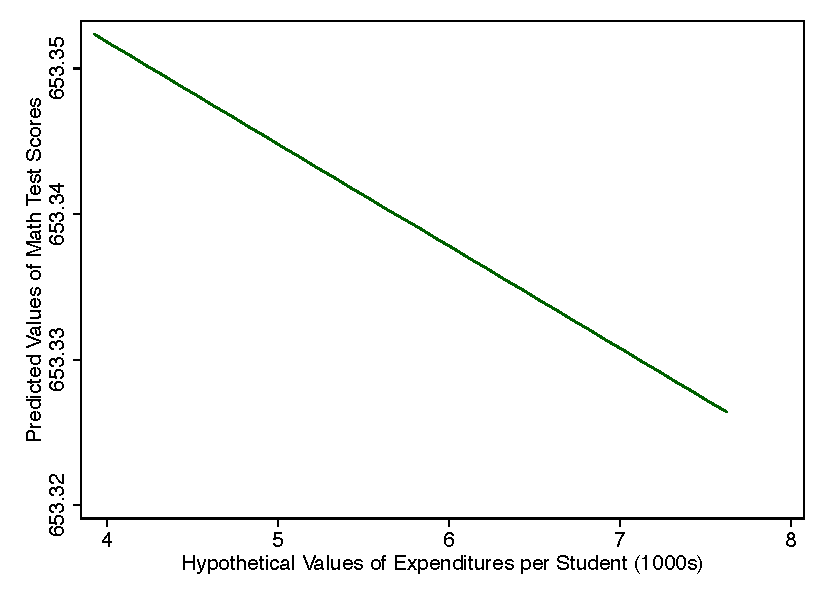
\includegraphics{basic_predict}
\end{figure}

Remember that the prediction interval does not tell us where we can
expect any individual unit to be located. Instead, the prediction
interval tells us the likely range of \emph{lines} that would be
generated in repeated samples. 

\subsection{Hypothetical Values}
\label{sec:hypothetical-values}

Many times, we'd also like to think about how the dependent variable
would increase or decrease as a function of hypothetical values of x.
Using only Stata's \texttt{predict} command, we're stuck with just
using the data in memory. The \texttt{margins} command can help us to
make predictions for hypothetical values of the independent variable. 

There are two steps to using margins. First, we need to generate
values of $\hat{y}$ across levels of x, then we need to generate the
standard error of $\hat{y}$ across those same levels of x. With those
estimates in hand, we can save them in memory and plot them. 

\begin{stlog}
  
. /*Making use of the margins command*/
. 
. 
. // Use summary to get min and max of key IV    
. sum `x', detail
. 
. local mymin=r(min)
. local mymax=r(max)
. 
. estimates restore basic_controls
. 
. local dfr=e(df_r)
. 
. #delimit ;
delimiter now ;
. margins , /* init margins */
>     predict(xb) /* Type of prediction */
>     nose /* Don't give SE */
>     at( (mean) /* Precition at mean of all variables */
>     `controls' /* Set controls at mean */
>     `x'=(`mymin'(.1)`mymax'))  /*range from min to max of x in steps of .1 *
> /
>      post  /* Post results in matrix form */
>          ;
. #delimit cr
delimiter now cr
. 
. // Pull results
. mat xb=e(b)
. 
. // store x values used to generate predictions
. mat allx=e(at)
. 
. // store just x values from that matrix
. matrix myx=allx[1...,1]'
. 
. // Bring back in regression results
. estimates restore basic_controls
. 
. // Run margins again, but this time get standard error of prediction as outp
> ut
. margins , predict(stdp) nose at(`x'=(`mymin'(.1)`mymax') (mean) `controls') 
> post
. 
. //Grab standard error of prediction
. mat stdp=e(b)
. 
. //Put three matrices together: standard error, prediction, and values of x: 
> transpose 
. mat pred1=[stdp \ xb\ myx]'
. 
. //Put matrix in data 
. svmat pred1
. 
. //Generate
. generate lb = pred12 - (`myt' * pred11) /*Prediction minus t value times SE 
> */
. generate ub = pred12 + (`myt'* pred11) /*Prediction plus t value times SE */
. 
. 
\end{stlog}

This gives us the following plot:

\begin{figure}
  \centering
  \caption{Predicted Value of Math Scores Across Hypothetical Levels
    of Student Teacher Ratio}
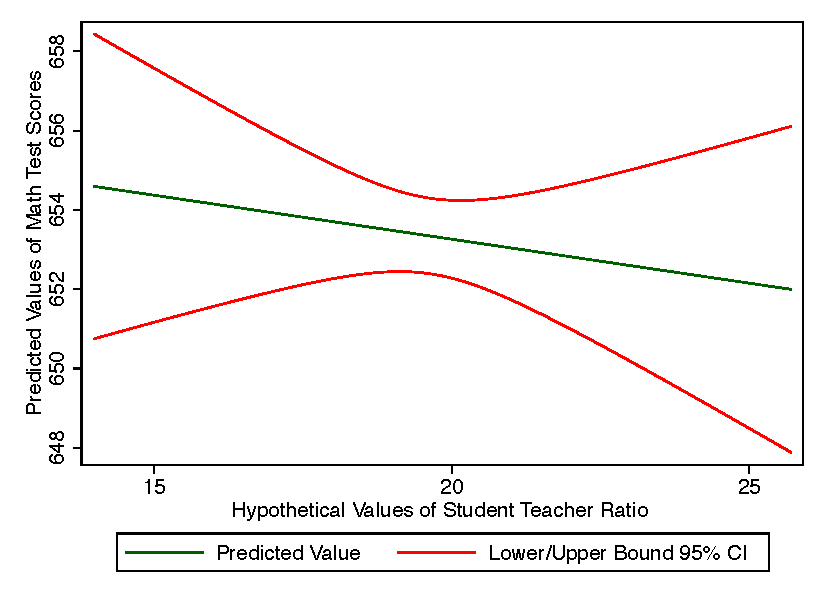
\includegraphics{ci_predict95}
\end{figure}



\section{Forecast Intervals}
\label{sec:forecast-intervals}

Forecasting is distinct from prediction in the parlance of
regression. The prediction interval is all about how different the
regression line is likely to be in repeated samples. The forecast
interval is all about how well the model predicts the location of
individual points. A 95\% confidence interval around the regression
line says: ``In 95 percent of repeated samples, an interval calculated
in this way will include the true value of the regression line.'' A
95\% forecast interval around the regression line says ``In 95 percent
of repeated samples, an interval calculated in this way will include
all but 5 percent of observations.'' 

The process for generating these lines is very similar to the one we
just went through, with the exception that we'll be using
\texttt{stdf}, the standrad error of the forecast, as opposed to
\texttt{stdp}, the standard error of the prediction. 

Here's what the forecast interval looks like for us, when predicting
using available data:


\begin{figure}
  \centering
  \caption{Predicted Value of Math Scores Across Levels
    of Student Teacher Ratio, Prediction vs. Forecasting}
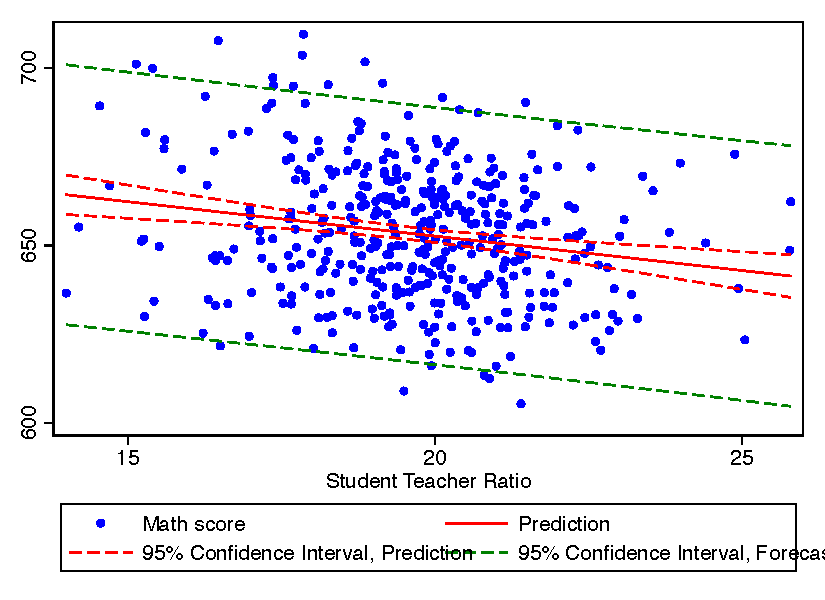
\includegraphics{predictvforecast}
\end{figure}

With hypothetical data, we're forecasting out of range, and so the
intervals are going to be quite wide. 

\begin{figure}
  \centering
  \caption{Predicted Value of Math Scores Across Hypothetical Levels
    of Student Teacher Ratio, Forecast Interval}
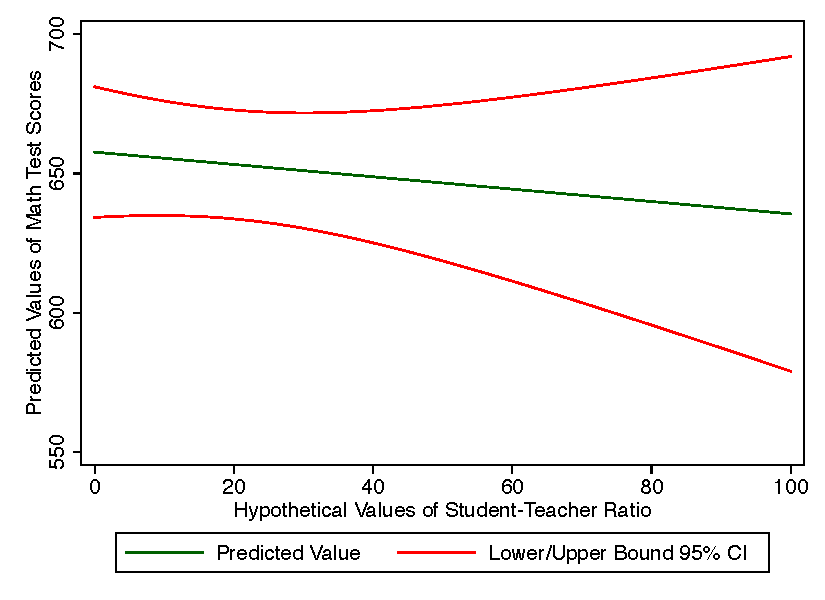
\includegraphics{ci_predict95_forecast}
\end{figure}

The point is that we should approach these results with some
humility. Too often, we don't take forecast intervals very
seriously. Predictions are made on ``average'' using the conditional
expectation function. If you're going to forecast for an individual
unit--- a person, a school, a state--- you need to acknowledge that
the uncertainty is likely to be large. 

\end{document}